\chapter{Vorgehensweise} 
Im folgenden Kapitel beschäftige ich mich mit der Ausarbeitung theoretischer Grundlagen als auch mit der groben Planung des Algorithmus und deren Komponenten.
\section{Überblick zum genetischen Algorithmus}
Genetische Algorithmen versuchen die Prozesse der natürlichen Evolution nachzuahmen. Dabei wird initial eine Population von potenziellen Lösungen erstellt, die durch eine Fitness Funktion bewertet wird. Ein guter Wert bei der Fitnessfunktion bedeutet eine gute Lösung. Mittels einer Selektion werden schlechtere Lösungen entfernt, sodass durch eine Kombination mehrerer guter Lösungen wieder bessere entstehen können. Um eine große Diversität zu gewährleisten, geschieht noch eine Mutation die Merkmale verschiebt. 
\section{Hyperparameter in neuronalen Netzen}
Hyperparameter sind Parameter welche den Lernprozess betreffen. Im Kontrast zu den Modellparametern, die während des Trainings aufgebaut werden, sind Hyperparameter beim Training bereits bekannt. Es gibt viele neuronale Netze die Erfolg mit dynamischen Parametern haben \parencite{schaul_no_2013}. Andere typische Hyperparameter eines neuronalen Netzes beinhaltet die Batch Größe, Anzahl von Epochen, als auch die Anzahl von Neuronen in der verdeckten Schicht. In dieser Hausarbeit beschränke ich mich auf die genannten Parameter.
\section{Aufbau des Genetischen Algorithmus}
Im nachfolgenden Kapitel beschäftige ich mich mit der Planung des genetischen Algorithmus, dabei wird auf die einzelnen Operationen eingegangen.
\subsection{Chromosome}
Ein Chromosome wird üblicherweise in binärer Darstellung kodiert. Dies hat den Vorteil das bitweise Operationen sehr effizient und schnell umsetzbar sind, allerdings kann dies auch zu Problemen führen. Bei der Mutation oder der Rekombination muss daher geachtet werden, dass die höher signifikanten Bits (MSB) der Zahl die Zahl unter Umständen extremst verändern. Um diese Nicht Linearität zu vermeiden müssen die Operationen besser angepasst werden \parencite{herrera_tackling_1998}.  

Ein Chromosom besteht aus 4 Parametern: Batch Größe,  Neuronen in der verdeckten Schicht, Anzahl von Epochen und der Lernrate. Da die geplante Rekombination mit Operationen auf reellen und natürlichen Zahlen durchführt werden, wurde sich gegen eine Repräsentation in Binärform entschieden. Bis auf die Lernrate werden alle Parameter als natürlich Zahl geführt.
\subsection{Population}
Initial wird eine Startpopulation erzeugt, dabei wird aus einen vorher definierten Bereich zufällig eine Zahl gewählt
\begin{itemize}
	\item \textbf{Lern Rate}: Es wird eine logarithmische Verteilung im Wertebereich von \(\left[ 0.1, 0.00001 \right]\) vorgenommen. Eine nicht logarithmische Verteilung ist hierbei nicht gewünscht, da die Lernrate ansonsten in aller Regel sehr nah an \textit{0.1} bleibt. Eine logarithmische Verteilung garantiert hier eine ausgeglichene Verteilung.
	\item \textbf{Batch Größe}: Stetige Gleichverteilung im natürlichen Intervall \(\left[ 8, 512 \right]\). 
	\item \textbf{Epochen}: Stetige Gleichverteilung im natürlichen Intervall \(\left[ 5, 20 \right]\). 
	\item \textbf{Neuronen in der verdeckten Schicht}: Stetige Gleichverteilung im natürlichen Intervall \(\left[ 10, 1000 \right]\). 
\end{itemize}
Durch erste Tests konnte eine maximale Konfiguration mit einer Batch Größe von 512 und 1000 Neuronen in der verdeckten Schicht ermittelt werden. Eine größere Konfiguration ist mit der aktuell verwendeten Hardware nicht möglich, da der Grafikspeicher nicht ausreichend groß ist.

\subsection{Fitness}
Bewertet eine mögliche Konfiguration an Hyperparametern innerhalb des neuronalen Netzes. Hierfür wird das neuronale Netz mit Daten trainiert und anschließend mit ungesehenen Daten validiert. Die Fehlerfunktion ("Loss"), auf Basis der Validierungsdaten, ist dabei ein guter Indikator für ein gut trainiertes Netz, denn anders als die Genauigkeit, welche nur ein metrischer Wert ist, reflektiert die Fehlerfunktion auch bei kleinen Änderungen im Netz einen niedrigeren Wert. Daher gilt es diese Funktion zu minimieren \parencite[Kapitel~4.3]{goodfellow_deep_2016}. 
\subsection{Selektion}
Um bereits gefundene lokale Optimas nicht zu verlieren, wird pro Generation jeweils 2 Elitisten bestimmt, diese werden unverändert in die nächste Generation übernommen. Zusätzlich findet ein Turnierselektion zwischen zwei Chromosomen statt. Der Gewinner kommt in die nächste Generation, ein erneutes Auswählen findet nicht statt. So können auch schlechtere Chromosomen in die nächste Generation kommen, sodass lokale Optimas besser umgangen werden können. Durch die Turnier Selektion wird die Population um 50\% reduziert.
\subsection{Rekombination}
Die Rekombination erfolgt über zwei Elternteile. Hierfür wird im Wertebereich des Parameters eine Normalverteilung zwischen den zwei Elternteilen formiert. So sind Werte innerhalb der beiden Elternteile wahrscheinlich, nicht aber zwangsläufig verpflichtend. Durch einen Parameter kann die Standardabweichung beeinflusst werden. So kann ein Fokus entweder auf Exploitation oder Exploration gelegt werden. Diese Art von Rekombination ist inspiriert durch die Gauss-Mutation \parencite[Seite~8]{kruse_evolutionare_2013}. 
\begin{figure}[h]
	\centering
	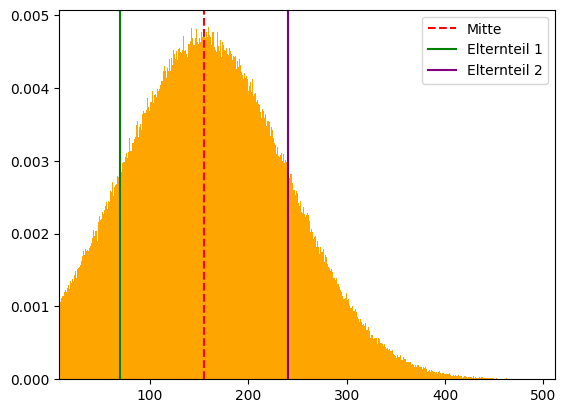
\includegraphics[width=1\linewidth]{rekombination.png}
	\caption{Normalverteilung bei der Rekombination für Batch Größe}
	\label{fig:enter-label}
\end{figure}

\subsection{Mutation}
Die Mutation findet an jeden Merkmal eines Chromosomes einzelnd statt. Mit einer Wahrscheinlichkeit von \textit{0,2} wird das Merkmal komplett neu gewürfelt. Dies erhöht die Diversität der Population und erweitert die Exploration.
\section{Bemerkungen zum Ansatz}
Der hier gewählte Ansatz hat seine eigenen Tücken, so ist die Wahl der Standardabweichung bei der Rekombination sehr wichtig um eine Balance zwischen Exploration und Exploitation zu finden. 